
% Default to the notebook output style

    


% Inherit from the specified cell style.




    
\documentclass[11pt]{article}

    
    
    \usepackage[T1]{fontenc}
    % Nicer default font than Computer Modern for most use cases
    \usepackage{palatino}

    % Basic figure setup, for now with no caption control since it's done
    % automatically by Pandoc (which extracts ![](path) syntax from Markdown).
    \usepackage{graphicx}
    % We will generate all images so they have a width \maxwidth. This means
    % that they will get their normal width if they fit onto the page, but
    % are scaled down if they would overflow the margins.
    \makeatletter
    \def\maxwidth{\ifdim\Gin@nat@width>\linewidth\linewidth
    \else\Gin@nat@width\fi}
    \makeatother
    \let\Oldincludegraphics\includegraphics
    % Set max figure width to be 80% of text width, for now hardcoded.
    \renewcommand{\includegraphics}[1]{\Oldincludegraphics[width=.8\maxwidth]{#1}}
    % Ensure that by default, figures have no caption (until we provide a
    % proper Figure object with a Caption API and a way to capture that
    % in the conversion process - todo).
    \usepackage{caption}
    \DeclareCaptionLabelFormat{nolabel}{}
    \captionsetup{labelformat=nolabel}

    \usepackage{adjustbox} % Used to constrain images to a maximum size 
    \usepackage{xcolor} % Allow colors to be defined
    \usepackage{enumerate} % Needed for markdown enumerations to work
    \usepackage{geometry} % Used to adjust the document margins
    \usepackage{amsmath} % Equations
    \usepackage{amssymb} % Equations
    \usepackage{textcomp} % defines textquotesingle
    % Hack from http://tex.stackexchange.com/a/47451/13684:
    \AtBeginDocument{%
        \def\PYZsq{\textquotesingle}% Upright quotes in Pygmentized code
    }
    \usepackage{upquote} % Upright quotes for verbatim code
    \usepackage{eurosym} % defines \euro
    \usepackage[mathletters]{ucs} % Extended unicode (utf-8) support
    \usepackage[utf8x]{inputenc} % Allow utf-8 characters in the tex document
    \usepackage{fancyvrb} % verbatim replacement that allows latex
    \usepackage{grffile} % extends the file name processing of package graphics 
                         % to support a larger range 
    % The hyperref package gives us a pdf with properly built
    % internal navigation ('pdf bookmarks' for the table of contents,
    % internal cross-reference links, web links for URLs, etc.)
    \usepackage{hyperref}
    \usepackage{longtable} % longtable support required by pandoc >1.10
    \usepackage{booktabs}  % table support for pandoc > 1.12.2
    \usepackage[normalem]{ulem} % ulem is needed to support strikethroughs (\sout)
                                % normalem makes italics be italics, not underlines
    

    
    
    % Colors for the hyperref package
    \definecolor{urlcolor}{rgb}{0,.145,.698}
    \definecolor{linkcolor}{rgb}{.71,0.21,0.01}
    \definecolor{citecolor}{rgb}{.12,.54,.11}

    % ANSI colors
    \definecolor{ansi-black}{HTML}{3E424D}
    \definecolor{ansi-black-intense}{HTML}{282C36}
    \definecolor{ansi-red}{HTML}{E75C58}
    \definecolor{ansi-red-intense}{HTML}{B22B31}
    \definecolor{ansi-green}{HTML}{00A250}
    \definecolor{ansi-green-intense}{HTML}{007427}
    \definecolor{ansi-yellow}{HTML}{DDB62B}
    \definecolor{ansi-yellow-intense}{HTML}{B27D12}
    \definecolor{ansi-blue}{HTML}{208FFB}
    \definecolor{ansi-blue-intense}{HTML}{0065CA}
    \definecolor{ansi-magenta}{HTML}{D160C4}
    \definecolor{ansi-magenta-intense}{HTML}{A03196}
    \definecolor{ansi-cyan}{HTML}{60C6C8}
    \definecolor{ansi-cyan-intense}{HTML}{258F8F}
    \definecolor{ansi-white}{HTML}{C5C1B4}
    \definecolor{ansi-white-intense}{HTML}{A1A6B2}

    % commands and environments needed by pandoc snippets
    % extracted from the output of `pandoc -s`
    \providecommand{\tightlist}{%
      \setlength{\itemsep}{0pt}\setlength{\parskip}{0pt}}
    \DefineVerbatimEnvironment{Highlighting}{Verbatim}{commandchars=\\\{\}}
    % Add ',fontsize=\small' for more characters per line
    \newenvironment{Shaded}{}{}
    \newcommand{\KeywordTok}[1]{\textcolor[rgb]{0.00,0.44,0.13}{\textbf{{#1}}}}
    \newcommand{\DataTypeTok}[1]{\textcolor[rgb]{0.56,0.13,0.00}{{#1}}}
    \newcommand{\DecValTok}[1]{\textcolor[rgb]{0.25,0.63,0.44}{{#1}}}
    \newcommand{\BaseNTok}[1]{\textcolor[rgb]{0.25,0.63,0.44}{{#1}}}
    \newcommand{\FloatTok}[1]{\textcolor[rgb]{0.25,0.63,0.44}{{#1}}}
    \newcommand{\CharTok}[1]{\textcolor[rgb]{0.25,0.44,0.63}{{#1}}}
    \newcommand{\StringTok}[1]{\textcolor[rgb]{0.25,0.44,0.63}{{#1}}}
    \newcommand{\CommentTok}[1]{\textcolor[rgb]{0.38,0.63,0.69}{\textit{{#1}}}}
    \newcommand{\OtherTok}[1]{\textcolor[rgb]{0.00,0.44,0.13}{{#1}}}
    \newcommand{\AlertTok}[1]{\textcolor[rgb]{1.00,0.00,0.00}{\textbf{{#1}}}}
    \newcommand{\FunctionTok}[1]{\textcolor[rgb]{0.02,0.16,0.49}{{#1}}}
    \newcommand{\RegionMarkerTok}[1]{{#1}}
    \newcommand{\ErrorTok}[1]{\textcolor[rgb]{1.00,0.00,0.00}{\textbf{{#1}}}}
    \newcommand{\NormalTok}[1]{{#1}}
    
    % Additional commands for more recent versions of Pandoc
    \newcommand{\ConstantTok}[1]{\textcolor[rgb]{0.53,0.00,0.00}{{#1}}}
    \newcommand{\SpecialCharTok}[1]{\textcolor[rgb]{0.25,0.44,0.63}{{#1}}}
    \newcommand{\VerbatimStringTok}[1]{\textcolor[rgb]{0.25,0.44,0.63}{{#1}}}
    \newcommand{\SpecialStringTok}[1]{\textcolor[rgb]{0.73,0.40,0.53}{{#1}}}
    \newcommand{\ImportTok}[1]{{#1}}
    \newcommand{\DocumentationTok}[1]{\textcolor[rgb]{0.73,0.13,0.13}{\textit{{#1}}}}
    \newcommand{\AnnotationTok}[1]{\textcolor[rgb]{0.38,0.63,0.69}{\textbf{\textit{{#1}}}}}
    \newcommand{\CommentVarTok}[1]{\textcolor[rgb]{0.38,0.63,0.69}{\textbf{\textit{{#1}}}}}
    \newcommand{\VariableTok}[1]{\textcolor[rgb]{0.10,0.09,0.49}{{#1}}}
    \newcommand{\ControlFlowTok}[1]{\textcolor[rgb]{0.00,0.44,0.13}{\textbf{{#1}}}}
    \newcommand{\OperatorTok}[1]{\textcolor[rgb]{0.40,0.40,0.40}{{#1}}}
    \newcommand{\BuiltInTok}[1]{{#1}}
    \newcommand{\ExtensionTok}[1]{{#1}}
    \newcommand{\PreprocessorTok}[1]{\textcolor[rgb]{0.74,0.48,0.00}{{#1}}}
    \newcommand{\AttributeTok}[1]{\textcolor[rgb]{0.49,0.56,0.16}{{#1}}}
    \newcommand{\InformationTok}[1]{\textcolor[rgb]{0.38,0.63,0.69}{\textbf{\textit{{#1}}}}}
    \newcommand{\WarningTok}[1]{\textcolor[rgb]{0.38,0.63,0.69}{\textbf{\textit{{#1}}}}}
    
    
    % Define a nice break command that doesn't care if a line doesn't already
    % exist.
    \def\br{\hspace*{\fill} \\* }
    % Math Jax compatability definitions
    \def\gt{>}
    \def\lt{<}
    % Document parameters
    \title{transforming-data}
    
    
    

    % Pygments definitions
    
\makeatletter
\def\PY@reset{\let\PY@it=\relax \let\PY@bf=\relax%
    \let\PY@ul=\relax \let\PY@tc=\relax%
    \let\PY@bc=\relax \let\PY@ff=\relax}
\def\PY@tok#1{\csname PY@tok@#1\endcsname}
\def\PY@toks#1+{\ifx\relax#1\empty\else%
    \PY@tok{#1}\expandafter\PY@toks\fi}
\def\PY@do#1{\PY@bc{\PY@tc{\PY@ul{%
    \PY@it{\PY@bf{\PY@ff{#1}}}}}}}
\def\PY#1#2{\PY@reset\PY@toks#1+\relax+\PY@do{#2}}

\expandafter\def\csname PY@tok@sc\endcsname{\def\PY@tc##1{\textcolor[rgb]{0.73,0.13,0.13}{##1}}}
\expandafter\def\csname PY@tok@mi\endcsname{\def\PY@tc##1{\textcolor[rgb]{0.40,0.40,0.40}{##1}}}
\expandafter\def\csname PY@tok@cp\endcsname{\def\PY@tc##1{\textcolor[rgb]{0.74,0.48,0.00}{##1}}}
\expandafter\def\csname PY@tok@kt\endcsname{\def\PY@tc##1{\textcolor[rgb]{0.69,0.00,0.25}{##1}}}
\expandafter\def\csname PY@tok@kn\endcsname{\let\PY@bf=\textbf\def\PY@tc##1{\textcolor[rgb]{0.00,0.50,0.00}{##1}}}
\expandafter\def\csname PY@tok@nc\endcsname{\let\PY@bf=\textbf\def\PY@tc##1{\textcolor[rgb]{0.00,0.00,1.00}{##1}}}
\expandafter\def\csname PY@tok@ch\endcsname{\let\PY@it=\textit\def\PY@tc##1{\textcolor[rgb]{0.25,0.50,0.50}{##1}}}
\expandafter\def\csname PY@tok@nv\endcsname{\def\PY@tc##1{\textcolor[rgb]{0.10,0.09,0.49}{##1}}}
\expandafter\def\csname PY@tok@w\endcsname{\def\PY@tc##1{\textcolor[rgb]{0.73,0.73,0.73}{##1}}}
\expandafter\def\csname PY@tok@vc\endcsname{\def\PY@tc##1{\textcolor[rgb]{0.10,0.09,0.49}{##1}}}
\expandafter\def\csname PY@tok@cpf\endcsname{\let\PY@it=\textit\def\PY@tc##1{\textcolor[rgb]{0.25,0.50,0.50}{##1}}}
\expandafter\def\csname PY@tok@gu\endcsname{\let\PY@bf=\textbf\def\PY@tc##1{\textcolor[rgb]{0.50,0.00,0.50}{##1}}}
\expandafter\def\csname PY@tok@na\endcsname{\def\PY@tc##1{\textcolor[rgb]{0.49,0.56,0.16}{##1}}}
\expandafter\def\csname PY@tok@cm\endcsname{\let\PY@it=\textit\def\PY@tc##1{\textcolor[rgb]{0.25,0.50,0.50}{##1}}}
\expandafter\def\csname PY@tok@gd\endcsname{\def\PY@tc##1{\textcolor[rgb]{0.63,0.00,0.00}{##1}}}
\expandafter\def\csname PY@tok@ne\endcsname{\let\PY@bf=\textbf\def\PY@tc##1{\textcolor[rgb]{0.82,0.25,0.23}{##1}}}
\expandafter\def\csname PY@tok@nd\endcsname{\def\PY@tc##1{\textcolor[rgb]{0.67,0.13,1.00}{##1}}}
\expandafter\def\csname PY@tok@nn\endcsname{\let\PY@bf=\textbf\def\PY@tc##1{\textcolor[rgb]{0.00,0.00,1.00}{##1}}}
\expandafter\def\csname PY@tok@vi\endcsname{\def\PY@tc##1{\textcolor[rgb]{0.10,0.09,0.49}{##1}}}
\expandafter\def\csname PY@tok@vg\endcsname{\def\PY@tc##1{\textcolor[rgb]{0.10,0.09,0.49}{##1}}}
\expandafter\def\csname PY@tok@gs\endcsname{\let\PY@bf=\textbf}
\expandafter\def\csname PY@tok@gr\endcsname{\def\PY@tc##1{\textcolor[rgb]{1.00,0.00,0.00}{##1}}}
\expandafter\def\csname PY@tok@s2\endcsname{\def\PY@tc##1{\textcolor[rgb]{0.73,0.13,0.13}{##1}}}
\expandafter\def\csname PY@tok@sx\endcsname{\def\PY@tc##1{\textcolor[rgb]{0.00,0.50,0.00}{##1}}}
\expandafter\def\csname PY@tok@o\endcsname{\def\PY@tc##1{\textcolor[rgb]{0.40,0.40,0.40}{##1}}}
\expandafter\def\csname PY@tok@mf\endcsname{\def\PY@tc##1{\textcolor[rgb]{0.40,0.40,0.40}{##1}}}
\expandafter\def\csname PY@tok@ni\endcsname{\let\PY@bf=\textbf\def\PY@tc##1{\textcolor[rgb]{0.60,0.60,0.60}{##1}}}
\expandafter\def\csname PY@tok@nt\endcsname{\let\PY@bf=\textbf\def\PY@tc##1{\textcolor[rgb]{0.00,0.50,0.00}{##1}}}
\expandafter\def\csname PY@tok@err\endcsname{\def\PY@bc##1{\setlength{\fboxsep}{0pt}\fcolorbox[rgb]{1.00,0.00,0.00}{1,1,1}{\strut ##1}}}
\expandafter\def\csname PY@tok@c1\endcsname{\let\PY@it=\textit\def\PY@tc##1{\textcolor[rgb]{0.25,0.50,0.50}{##1}}}
\expandafter\def\csname PY@tok@ow\endcsname{\let\PY@bf=\textbf\def\PY@tc##1{\textcolor[rgb]{0.67,0.13,1.00}{##1}}}
\expandafter\def\csname PY@tok@sb\endcsname{\def\PY@tc##1{\textcolor[rgb]{0.73,0.13,0.13}{##1}}}
\expandafter\def\csname PY@tok@gh\endcsname{\let\PY@bf=\textbf\def\PY@tc##1{\textcolor[rgb]{0.00,0.00,0.50}{##1}}}
\expandafter\def\csname PY@tok@kr\endcsname{\let\PY@bf=\textbf\def\PY@tc##1{\textcolor[rgb]{0.00,0.50,0.00}{##1}}}
\expandafter\def\csname PY@tok@ge\endcsname{\let\PY@it=\textit}
\expandafter\def\csname PY@tok@sh\endcsname{\def\PY@tc##1{\textcolor[rgb]{0.73,0.13,0.13}{##1}}}
\expandafter\def\csname PY@tok@mh\endcsname{\def\PY@tc##1{\textcolor[rgb]{0.40,0.40,0.40}{##1}}}
\expandafter\def\csname PY@tok@no\endcsname{\def\PY@tc##1{\textcolor[rgb]{0.53,0.00,0.00}{##1}}}
\expandafter\def\csname PY@tok@kc\endcsname{\let\PY@bf=\textbf\def\PY@tc##1{\textcolor[rgb]{0.00,0.50,0.00}{##1}}}
\expandafter\def\csname PY@tok@s1\endcsname{\def\PY@tc##1{\textcolor[rgb]{0.73,0.13,0.13}{##1}}}
\expandafter\def\csname PY@tok@nb\endcsname{\def\PY@tc##1{\textcolor[rgb]{0.00,0.50,0.00}{##1}}}
\expandafter\def\csname PY@tok@cs\endcsname{\let\PY@it=\textit\def\PY@tc##1{\textcolor[rgb]{0.25,0.50,0.50}{##1}}}
\expandafter\def\csname PY@tok@ss\endcsname{\def\PY@tc##1{\textcolor[rgb]{0.10,0.09,0.49}{##1}}}
\expandafter\def\csname PY@tok@s\endcsname{\def\PY@tc##1{\textcolor[rgb]{0.73,0.13,0.13}{##1}}}
\expandafter\def\csname PY@tok@gt\endcsname{\def\PY@tc##1{\textcolor[rgb]{0.00,0.27,0.87}{##1}}}
\expandafter\def\csname PY@tok@nf\endcsname{\def\PY@tc##1{\textcolor[rgb]{0.00,0.00,1.00}{##1}}}
\expandafter\def\csname PY@tok@mb\endcsname{\def\PY@tc##1{\textcolor[rgb]{0.40,0.40,0.40}{##1}}}
\expandafter\def\csname PY@tok@nl\endcsname{\def\PY@tc##1{\textcolor[rgb]{0.63,0.63,0.00}{##1}}}
\expandafter\def\csname PY@tok@kd\endcsname{\let\PY@bf=\textbf\def\PY@tc##1{\textcolor[rgb]{0.00,0.50,0.00}{##1}}}
\expandafter\def\csname PY@tok@k\endcsname{\let\PY@bf=\textbf\def\PY@tc##1{\textcolor[rgb]{0.00,0.50,0.00}{##1}}}
\expandafter\def\csname PY@tok@kp\endcsname{\def\PY@tc##1{\textcolor[rgb]{0.00,0.50,0.00}{##1}}}
\expandafter\def\csname PY@tok@sr\endcsname{\def\PY@tc##1{\textcolor[rgb]{0.73,0.40,0.53}{##1}}}
\expandafter\def\csname PY@tok@gp\endcsname{\let\PY@bf=\textbf\def\PY@tc##1{\textcolor[rgb]{0.00,0.00,0.50}{##1}}}
\expandafter\def\csname PY@tok@c\endcsname{\let\PY@it=\textit\def\PY@tc##1{\textcolor[rgb]{0.25,0.50,0.50}{##1}}}
\expandafter\def\csname PY@tok@m\endcsname{\def\PY@tc##1{\textcolor[rgb]{0.40,0.40,0.40}{##1}}}
\expandafter\def\csname PY@tok@gi\endcsname{\def\PY@tc##1{\textcolor[rgb]{0.00,0.63,0.00}{##1}}}
\expandafter\def\csname PY@tok@go\endcsname{\def\PY@tc##1{\textcolor[rgb]{0.53,0.53,0.53}{##1}}}
\expandafter\def\csname PY@tok@si\endcsname{\let\PY@bf=\textbf\def\PY@tc##1{\textcolor[rgb]{0.73,0.40,0.53}{##1}}}
\expandafter\def\csname PY@tok@mo\endcsname{\def\PY@tc##1{\textcolor[rgb]{0.40,0.40,0.40}{##1}}}
\expandafter\def\csname PY@tok@il\endcsname{\def\PY@tc##1{\textcolor[rgb]{0.40,0.40,0.40}{##1}}}
\expandafter\def\csname PY@tok@bp\endcsname{\def\PY@tc##1{\textcolor[rgb]{0.00,0.50,0.00}{##1}}}
\expandafter\def\csname PY@tok@se\endcsname{\let\PY@bf=\textbf\def\PY@tc##1{\textcolor[rgb]{0.73,0.40,0.13}{##1}}}
\expandafter\def\csname PY@tok@sd\endcsname{\let\PY@it=\textit\def\PY@tc##1{\textcolor[rgb]{0.73,0.13,0.13}{##1}}}

\def\PYZbs{\char`\\}
\def\PYZus{\char`\_}
\def\PYZob{\char`\{}
\def\PYZcb{\char`\}}
\def\PYZca{\char`\^}
\def\PYZam{\char`\&}
\def\PYZlt{\char`\<}
\def\PYZgt{\char`\>}
\def\PYZsh{\char`\#}
\def\PYZpc{\char`\%}
\def\PYZdl{\char`\$}
\def\PYZhy{\char`\-}
\def\PYZsq{\char`\'}
\def\PYZdq{\char`\"}
\def\PYZti{\char`\~}
% for compatibility with earlier versions
\def\PYZat{@}
\def\PYZlb{[}
\def\PYZrb{]}
\makeatother


    % Exact colors from NB
    \definecolor{incolor}{rgb}{0.0, 0.0, 0.5}
    \definecolor{outcolor}{rgb}{0.545, 0.0, 0.0}



    
    % Prevent overflowing lines due to hard-to-break entities
    \sloppy 
    % Setup hyperref package
    \hypersetup{
      breaklinks=true,  % so long urls are correctly broken across lines
      colorlinks=true,
      urlcolor=urlcolor,
      linkcolor=linkcolor,
      citecolor=citecolor,
      }
    % Slightly bigger margins than the latex defaults
    
    \geometry{verbose,tmargin=1in,bmargin=1in,lmargin=1in,rmargin=1in}
    
    

    \begin{document}
    
    
    \maketitle
    
    

    
    \subsection{Transforming Data}\label{transforming-data}

Your goal during the data gathering phase is to record as much working
data about your observations as possible since you never know which
feature is going to end up being the golden one that allows your machine
learning algorithm to succeed. Due to this, there are usually a few
redundant or even poor features in your dataset. Think back to those
long word problems in grade school that were essentially a simple math
question, but came filled with red herrings to throw you off; feeding an
unfiltered soup of features to your machine learning algorithms is
pretty similar to trying to get it to solve those word problems.

To be effective, many machine learning algorithms need the data passed
to them be discerning, discriminating and independent. In this module,
you're going to discover methods to get your data behaving like that
using transformers. This will help improve your own knowledge of your
data, as well as improve your machine learning algorithms' performance.

A transformer is any algorithm you apply to your dataset that changes
either the feature count or feature values, but does not alter the
number of observations. You can use transformers to mung your data as a
pre-processing step to clean it up before it's fed to other algorithms.
Another popular transformer use is that of dimensionality reduction,
where the number of features in your dataset is intelligently reduced to
a subset of the original.

Once you've used a few basic transformers, you will also learn about
some data cleansing techniques that attempt to rectify problematic
observations.

    \subsubsection{Principal Component Analysis
(PCA)}\label{principal-component-analysis-pca}

Unsupervised learning aims to discover some type of hidden structure
within your data. Without a label or correct answer to test against,
there is no metric for evaluating unsupervised learning algorithms.
Principal Component Analysis (PCA), a transformation that attempts to
convert your possibly correlated features into a set of linearly
uncorrelated ones, is the first unsupervised learning algorithm you'll
study.

\paragraph{What is principal component
analysis}\label{what-is-principal-component-analysis}

\textbf{PCA falls into the group of dimensionality reduction
algorithms}. \emph{In many real-world datasets and the problems they
represent, you aren't aware of what specifically needs to be measured to
succinctly address the issue driving your data collection. So instead,
you simply record any feature you can derive, usually resulting in a
higher dimensionality than what is truly needed}. This is undesirable,
but it's the only reliable way you know to insure you capture the
relationship modeled in your data.

If you have reason to believe \emph{your question has a simple answer},
or that \emph{the features you've collected are actually many indirect
observations of some inherent source you either cannot or do not know
how to measure}, then \textbf{dimensionality reduction applies to your
needs}.

\textbf{PCA's approach} to \emph{dimensionality reduction} is to
\textbf{derive a set of degrees of freedom that can then be used to
reproduce most of the variability of your data}. Picture one of those
cartoon style telephone poles; once you have a figure in mind, compare
it to this one:

\begin{figure}
\centering

\includegraphics{pic/telephone.png}
\caption{telephone-front-view}
\end{figure}

Your envisioned image probably looked similar. You could have pictured
it from any other viewing angle, for instance, as if you were floating
directly above it looking down:

\begin{figure}
\centering

\includegraphics{pic/telephone-above.png}
\caption{telephone-above-view}
\end{figure}

However you probably didn't, since that view doesn't contain enough
variance, or information to easily be discernible as a telephone pole.
The frontal view, however, does. Looking at a telephone pole or any
other object from various viewing angles gives you more information
about that object. If the view angles are really close to one another,
the information you get from the views ends up being mostly the same,
with a lot of duplicate information. However if you're able to move to a
completely different angle, you can get a lot more information about the
object you're examining. And if you're wise in choose your view angles,
with just a few calculated glimpses of an object, you can build a rather
comprehensive understanding of it. PCA calculates those best view
angles:

\begin{figure}
\centering
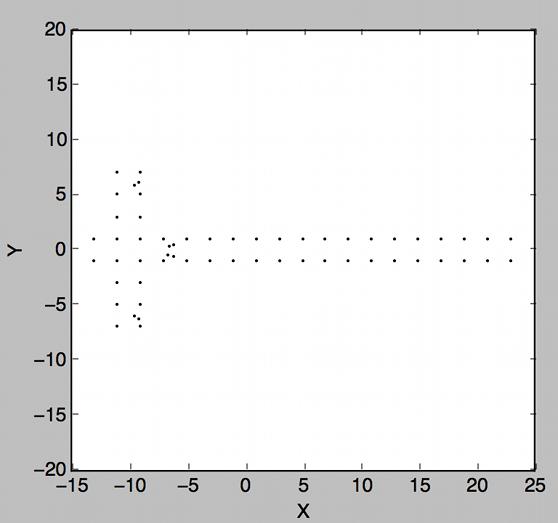
\includegraphics{pic/telephone-best-view.png}
\caption{telephone-best-view}
\end{figure}

\paragraph{How Does PCA Work?}\label{how-does-pca-work}

\textbf{PCA is one of the most popular techniques for dimensionality
reduction}, and \emph{we recommend you always start with it when you
have a complex dataset}. \textbf{It models a linear subspace of your
data by capturing its greatest variability}. Stated differently,
\textbf{it accesses your dataset's covariance structure directly using
matrix calculations and eigenvectors to compute the best unique features
that describe your samples}.

An iterative approach to this would \textbf{first find the center of
your data}, \emph{based off its numeric features}. Next, it would
\textbf{search for the direction that has the most variance or widest
spread of values}. \emph{That direction is the principal component
vector, so it is then added to a list}. By \textbf{searching for more
directions of maximal variance that are orthogonal to all previously
computed vectors}, \emph{more principal component can then be added to
the list}. \textbf{This set of vectors form a new feature space that you
can represent your samples with}.

\subparagraph{On Dimensions, Features, and
Views}\label{on-dimensions-features-and-views}

Each sample in your dataset represents an observable phenomenon, such as
an object in the real world. Each feature in your dataset tells you
details about your samples. \textbf{Recall from earlier chapters that
features and views are synonymous terms; this isn't accidental!} Just
like looking at an object from different views gives you more
information about the object, so too does examining a sample from
different features. Similar or correlated features will produce an
``overlapped'' view of your samples, the same way similar views of an
object also overlap.

\textbf{PCA ensures that each newly computed view (feature) is
orthogonal or linearly independent to all previously computed ones,
minimizing these overlaps}. PCA also orders the features by importance,
assuming that the more variance expressed in a feature, the more
important it is. In our telephone pole example, the frontal view had
more variance than the bird's-eye view and so it was preferred by PCA.

\begin{figure}
\centering
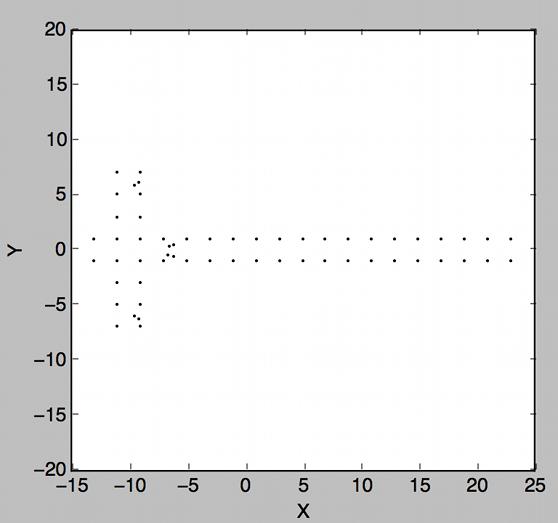
\includegraphics{pic/telephone-best-view.png}
\caption{telephone-best-view}
\end{figure}

\emph{With the \textbf{newly computed features ordered by importance,
dropping the least important features on the list intelligently reduces
the number of dimensions needed to represent your dataset}, with minimal
loss of information}. This has many practical uses, including boiling
off high dimensionality observations to just a few key dimensions for
visualization purposes, being used as a noise removal mechanism, and as
a pre-processing step before sending your data through to other more
processor-intensive algorithms. We'll look at more real life use cases
in the next unit.

\paragraph{When should I use PCA?}\label{when-should-i-use-pca}

PCA, and in fact all dimesionality reduction methods, have three main
uses: + To handle the clear goal of reducing the dimensionality and thus
complexity of your dataset. + To pre-process your data preparation for
other supervised learning tasks, suchs as regression and classification.
+ To make visualizing your data easier, since we can only preceive three
dimensions simultaneously.

According to Nielson Tetrad Demographics, the group of people who watch
the most movies are people between the ages of 24 through 35. Let's say
you had a list of 100 movies and surveyed 5000 people from within this
demographic, asking them to rate all the movies they've seen on a scale
of 1-10. By having considerably more data samples (5000 people) than
features (100 ordinal movie ratings), you're more likely to avoid the
\href{https://en.wikipedia.org/wiki/Curse_of_dimensionality}{curse of
dimensionality}.

Having collected all that data, even though you asked 100 questions,
what do you think truly is being measured by the survey? Overall, it is
the collective movie preference per person. You could attempt to solve
for this manually in a supervised way, by break down movies into
well-known genres: + Action + Adventure + Comedy + Crime \& Gangster +
Drama + Historical + Horror + Musicals + Science Fiction + War + Western
+ etc.

Being unsupervised, PCA doesn't have access to these genre labels. In
fact, it doesn't have or care for any labels whatsoever. This is
important because it's entirely possible there wasn't a single western
movie in your list of 1000 films, so it would be inappropriate and
strange for PCA to derive a `Western' principal component feature. By
using PCA, rather than you creating categories manually, it discovers
the natural categories that exist in your data. It can find as many of
them as you tell it to, so long as that number is less than the original
number of features you provided, and as long as you have enough samples
to support it. The groups it finds are the principal components, and
they are the best possible, linearly independent combination of features
that you can use to describe your data.

Being unsupervised, PCA doesn't have access to these genre labels. In
fact, it doesn't have or care for any labels whatsoever. This is
important because it's entirely possible there wasn't a single western
movie in your list of 1000 films, so it would be inappropriate and
strange for PCA to derive a `Western' principal component feature. By
using PCA, rather than you creating categories manually, it discovers
the natural categories that exist in your data. It can find as many of
them as you tell it to, so long as that number is less than the original
number of features you provided, and as long as you have enough samples
to support it. The groups it finds are the principal components, and
they are the best possible, linearly independent combination of features
that you can use to describe your data.

One warning is that again, being unsupervised, PCA can't tell you
exactly know what the newly created components or features mean. If
you're interested in how to interpret your principal components, we've
included two sources in the dive deeper section to help out with that
and highly recommend you explore them.

Once you've reduced your dataset's dimensionality using PCA to best
describe its variance and linear structure, you can then transform your
movie questionnaire dataset from its original {[}1000, 100{]}
feature-space into the much more comfortable, principal component space,
such as {[}1000, 10{]}. You can visualize your samples in this new space
using an Andrew's plot, or scatter plot. And finally, you can base the
rest of your analysis on your transformed features, rather than the
original 100 feature dataset.

PCA is a very fast algorithm and helps you vaporizes redundant features,
so when you have a high dimensionality dataset, start by running PCA on
it and then visualizing it. This will better help you understand your
data before continuing.

\subparagraph{Projecting a Shadow}\label{projecting-a-shadow}

By transforming your samples into the feature space created by
discarding under-prioritized features, a lower dimensional
representation of your data, also known as \textbf{shadow} or
\textbf{projection} is formed. In the shadow, some information has been
lost---it has fewer features after all. You can actually visualize how
much information has been lost by taking each sample and moving it to
the nearest spot on the projection feature space. In the following 2D
dataset, the orange line represents the principal component direction,
and the gray line represents the second principal component. The one
that's going to get dropped:

\begin{figure}
\centering
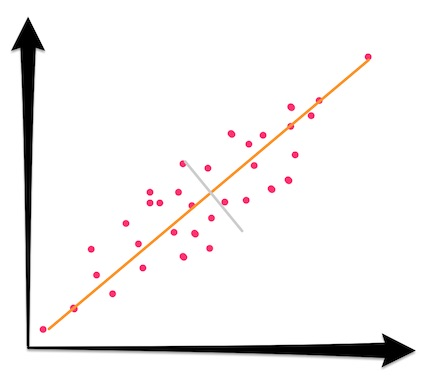
\includegraphics{pic/pca-projection-shadow.png}
\caption{pca-projection-shadow}
\end{figure}

By dropping the gray component above, the goal is to project the 2D
points onto 1D space. Move the original 2D samples to their closest spot
on the line:

\begin{figure}
\centering
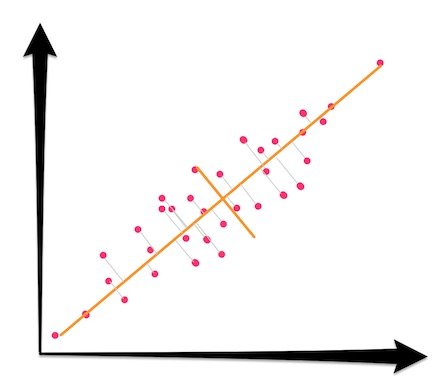
\includegraphics{pic/pca-projection-shadow2.png}
\caption{pca-projection-shadow2}
\end{figure}

Once you've projected all samples to their closest spot on the major
principal component, a shadow, or lower dimensional representation has
been formed:

\begin{figure}
\centering
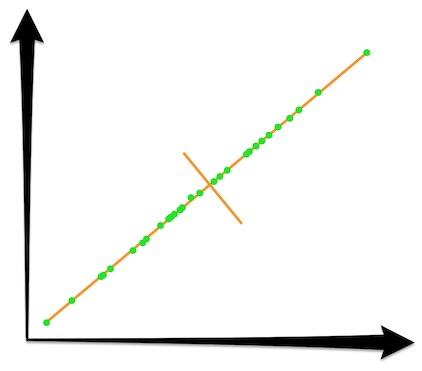
\includegraphics{pic/pca-projection-shadow3.png}
\caption{pca-projection-shadow3}
\end{figure}

The summed distances traveled by all moved samples is equal to the total
information lost by the projection. An an ideal situation, this lost
information should be dominated by highly redundant features and random
noise.

\paragraph{SciKit-Learn and PCA}\label{scikit-learn-and-pca}

To get started, import PCA from \texttt{sklearn.decomposition} and then
create a new instance of the model setting the
\texttt{n\_components\ parameter} to the number of dimensions you wish
to keep. This value has to be less than or equal to the number of
features in your original dataset, since each computed component is a
linear combination of your original features:

    \begin{Verbatim}[commandchars=\\\{\}]
{\color{incolor}In [{\color{incolor}6}]:} \PY{k+kn}{import} \PY{n+nn}{pandas} \PY{k}{as} \PY{n+nn}{pd}
        \PY{k+kn}{from} \PY{n+nn}{sklearn}\PY{n+nn}{.}\PY{n+nn}{decomposition} \PY{k}{import} \PY{n}{PCA}
        
        \PY{n}{df} \PY{o}{=} \PY{n}{pd}\PY{o}{.}\PY{n}{read\PYZus{}csv}\PY{p}{(}\PY{l+s+s2}{\PYZdq{}}\PY{l+s+s2}{Datasets/students.data}\PY{l+s+s2}{\PYZdq{}}\PY{p}{)}
        
        \PY{n}{pca} \PY{o}{=} \PY{n}{PCA}\PY{p}{(}\PY{n}{n\PYZus{}components}\PY{o}{=}\PY{l+m+mi}{2}\PY{p}{)}
        \PY{n}{pca}\PY{o}{.}\PY{n}{fit}\PY{p}{(}\PY{n}{df}\PY{p}{)}
        \PY{n+nb}{print} \PY{p}{(}\PY{n}{pca}\PY{p}{)}
        
        \PY{n}{T} \PY{o}{=} \PY{n}{pca}\PY{o}{.}\PY{n}{transform}\PY{p}{(}\PY{n}{df}\PY{p}{)} 
        
        \PY{n+nb}{print} \PY{p}{(}\PY{n}{df}\PY{o}{.}\PY{n}{shape}\PY{p}{)} \PY{c+c1}{\PYZsh{} (430, 6) \PYZhy{} 430 Student survey responses, 6 questions..}
        \PY{n+nb}{print} \PY{p}{(}\PY{n}{T}\PY{o}{.}\PY{n}{shape}\PY{p}{)} \PY{c+c1}{\PYZsh{} (430, 2) \PYZhy{} 430 Student survey responses, 2 principal components}
\end{Verbatim}

    \begin{Verbatim}[commandchars=\\\{\}]
PCA(copy=True, n\_components=2, whiten=False)
(649, 29)
(649, 2)

    \end{Verbatim}

    Once you've fit the model against your dataframe, you can use it to
transform your dataset's observations (or any other observation that
share its feature space) into the newly computed, principal component
feature space with the \texttt{.transform()} method. This transformation
is bidirectional, so you can recover your original feature values using
\texttt{.inverse\_transform()} so long as you don't drop any components.
If even one component was removed, then after performing the inverse
transformation back to the regular feature space, there will be some
signs of information loss proportional to which component was dropped.

There are a few other interesting model attribute that SciKit-Learn
exposes to you after you've trained your PCA model with the
\texttt{.fit()} method:

\begin{itemize}
\tightlist
\item
  \textbf{\texttt{components\_}} These are your principal component
  vectors and are linear combinations of your original features. As
  such, they exist within the feature space of your original dataset.
\item
  \textbf{\texttt{explained\_variance\_}} This is the calculated amount
  of variance which exists in the newly computed principal components.
\item
  \textbf{\texttt{explained\_variance\_ratio\_}} Normalized version of
  \texttt{explained\_variance\_} for when your interest is with
  probabilities.
\end{itemize}

\paragraph{PCA Gotchas!}\label{pca-gotchas}

To use PCA effectively, you should be aware of its weaknesses. The first
is that \textbf{PCA is sensitive to the scaling of your features}. PCA
maximizes variability based off of variance (the average squared
differences of your samples from the mean), and then projects your
original data on these directions of maximal variance. If your has a
feature with a large variance and others with small variances, PCA will
load on the larger variance feature. Being a linear transformation, it
will rotate and reorient your feature space so it diverts as much of the
variance of the larger-variance feature (and some of the other features'
variances), into the first few principal components.

When it does this, a feature might go from having little impact on your
transformation to totally dominating the first principal component, or
vice versa. \textbf{Standardizing your variables ahead of time is the
way to free your PCA results of such scaling issues}. \emph{The cases
where you should not use standardization are when you know your feature
variables, and thus their importance, need to respect the specific
scaling you've set up}. In such a case, PCA would be used on your raw
data.

PCA is extremely fast, but for very large datasets it might take a while
to train. All of the matrix computations required for inversion,
eigenvalue decomposition, etc. boggle it down. Since most real-world
datasets are typically very large and will have a level of noise in
them, razor-sharp, machine-precision matrix operations aren't always
necessary. If you're willing to sacrifice a bit of accuracy for
computational efficiency, \emph{SciKit-Learn offers a sister algorithm
called \textbf{RandomizedPCA} that applies some approximation techniques
to speed up large-scale matrix computation}. You can use this for your
larger datasets.

\textbf{The last issue to keep in mind is that PCA is a linear
transformation only}! In graphical terms, it can rotate and translate
the feature space of your samples, but will not skew them. \emph{PCA
will only, therefore, be able to capture the underlying linear shapes
and variance within your data and cannot discern any complex, nonlinear
intricacies. For such cases, you will have to make use different
dimensionality reduction algorithms, such as \textbf{Isomap}}.

\paragraph{Knowledge checks}\label{knowledge-checks}

\subparagraph{Review Question 1}\label{review-question-1}

1/1 point (graded)

Please complete the sentence so that it makes the most sense:

Principal component analysis\ldots{}

\begin{itemize}
\tightlist
\item
  Requires you have labeled features to use as a metric for determining
  which features are most important
\item
  Is a dimensionality reduction technique that builds a simpler,
  non-linear projection or `shadow' of your dataset
\item
  Asserts you have more features than samples so you can avoid the curse
  of dimensionality and the matrix math works out
\item
  Ensures each newly computed feature is orthogonal to all previously
  computed ones, minimizing overlaps
\end{itemize}

\emph{Answer:} \textbf{D} \#\#\#\#\# Review Question 2 1 point possible
(graded)

Which of these statements is wrong?

\begin{itemize}
\tightlist
\item
  PCA can be used to discover the underlying features being assessed by
  a dataset
\item
  The results of PCA depend on the scaling of your data, so having a
  feature with units of `light-years' and another feature with units of
  `GHz' may be disastrous
\item
  When applied to non-linear data, PCA generally isn't as effective as
  when applied to linear data
\item
  Since PCA is sensitive to feature scaling, if you have a feature that
  is a linear transformation of the other, e.g.~feature2 = 10 *
  feature1, then both features will be ignored
\end{itemize}

\emph{Answer:} \textbf{D}

    \subsubsection{PCA Lab}\label{pca-lab}

\paragraph{Assignment 1}\label{assignment-1}

\subparagraph{Lab Assignement 1}\label{lab-assignement-1}

In this assignment, you're going to experiment with a real life
armadillo sculpture scanned using a Cyberware 3030 MS 3D scanner at
Stanford University. The sculpture is available as part of their 3D
Scanning Repository, and is a very dense 3D mesh consisting of 172974
vertices! The mesh is available for you, located at
/Module4/Datasets/\textbf{stanford\_armadillo.ply}. It is \emph{not} a
Python file, so don't attempt to load it with a text editor!

\begin{figure}
\centering
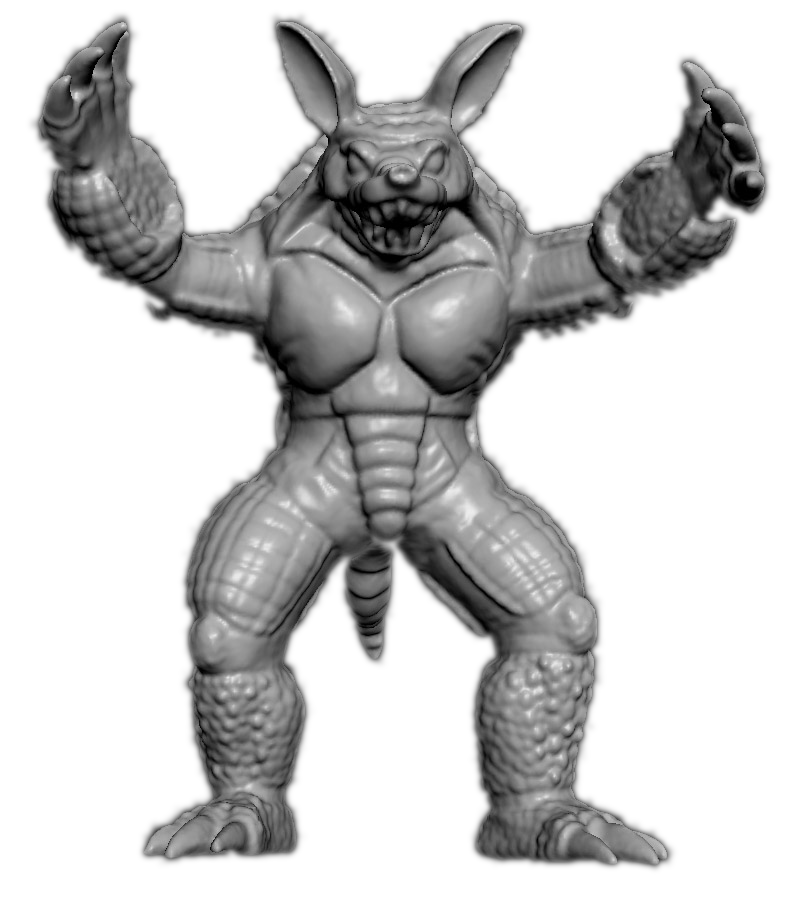
\includegraphics{pic/armadillo.png}
\caption{armadillo}
\end{figure}

Open up the Module4/\textbf{assignment1.py} starter code and read
through it carefully. You will notice the use of a new library, Plyfile.
This library loads up the 3D binary mesh for you. The mesh is further
converted into a Pandas dataframe for your ease of manipulation.
Complete the following tasks:

\begin{enumerate}
\def\labelenumi{\arabic{enumi}.}
\tightlist
\item
  Before changing any of the code, go ahead and execute assignment1.py.
  You should see the 3D armadillo. Your goal is to reduce its
  dimensionality from three to two using PCA to cast a shadow of the
  data onto its two most important principal components. Then render the
  resulting 2D scatter plot.
\item
  Fill out the proper code in the \texttt{do\_PCA()} and
  \texttt{do\_RandomizedPCA()} methods. Be sure to \textbf{return} the
  result of your transformation! You may even want to read the
  SciKit-Learn documentation on
  \href{http://scikit-learn.org/stable/modules/generated/sklearn.decomposition.PCA.html\#sklearn.decomposition.PCA.transform}{\texttt{.transform()}},
  just for future reference so you know what data type comes out of it.
\item
  Re-run the application! Then, answer the questions below:
\end{enumerate}

\subparagraph{Lab Question 1}\label{lab-question-1}

1 point possible (graded)

The first time you see the armadillo in 3D, what direction was its face
pointing towards?

\begin{itemize}
\tightlist
\item
  Left, Towards the negative X-Axis
\item
  Up, Towards the positive Z-Axis
\item
  Right, Towards the positive X-Axis
\item
  Down, Towards the negative Z-Axis
\end{itemize}

\emph{Answer:} \textbf{A} \#\#\#\#\# Lab Question 2 2 point possible
(graded)

Were you able to discern any \textbf{visual} differences between the
transformed PCA results and the transformed RandomizedPCA results?

\begin{itemize}
\tightlist
\item
  Yes, the RandomizedPCA version was no longer even recognizable as an
  armadillo
\item
  Yes, the RandomizedPCA version was a lot less true to the original
  than the regular PCA version
\item
  Yes, but it wasn't a lot\ldots{} just minor differences
\item
  No, they pretty much looked the same to me
\end{itemize}

Which executed faster, RandomizedPCA or PCA?

\begin{itemize}
\tightlist
\item
  PCA
\item
  RandomizedPCA
\end{itemize}

\emph{Answer:} \textbf{RandomizedPCA}

\subparagraph{Lab Assignement 2}\label{lab-assignement-2}

In Lab Assignment 1, you applied PCA to a dataset generated by
3D-scanning an actual sculpture. Real life 3D objects are a good segue
to PCA, since it's \textbf{fun} to see its effects on a dataset we can
see and touch. Another benefit is that all three spatial dimensions,
\textbf{x}, \textbf{y}, and \textbf{z}, each measure the same
unit-length relative to one another, so no extra consideration need be
made to account for PCA's weakness of requiring feature scaling.

But now the \textbf{fun} is over. Gaining some practical experience with
real-world datasets, which rarely allot you the luxury of having
features all on the same scale, will help you see how critical feature
scaling is to PCA. In this lab, you're going to experiment with a subset
of UCI's Chronic Kidney Disease data set, a collection of samples taken
from patients in India over a two month period, some of whom were in the
early stages of the disease. The starter code over at
/Module4/\textbf{assignment2.py}.

\begin{enumerate}
\def\labelenumi{\arabic{enumi}.}
\tightlist
\item
  Start by looking through the attribute information on the dataset
  website. Whenever you're given a dataset, the first thing you should
  do is find out as much about it as possible, both by reading up on any
  metadata, as well as by prodding through the actual data.
  Particularly, pay attention to what the docs say about these three
  variables: \textbf{bgr}, \textbf{rc}, and \textbf{wc}.
\item
  Load up the \textbf{\texttt{kidney\_disease.csv}} dataset from the
  /Module4/Datasets/ directory, and drop \textbf{all rows} that have
  \emph{any} nans. You're probably already a pro at doing that by now.
  In addition to getting rid of nans, did you know that the
  \texttt{.dropna()} method (upon completion) also automatically
  re-checks your features and assigns them an appropriate inferred data
  types?
\item
  Use an appropriate indexer command to select only the following
  columns: \textbf{bgr}, \textbf{rc}, and \textbf{wc}. Or alternatively,
  you can drop every other column, but it's probably easier to just use
  an indexer to select the one's you wish to keep.
\item
  Do a check of your dataframe's dtypes. Anything that didn't make it to
  the right type, you may want to investigate. Look through the data and
  identify \emph{why} the conversion failed. These types of problems
  often arise when you aren't in control of how your data is organized.
  Luckily the issue isn't too bad so once you've identified it, you can
  fix it through simple numeric coercion.
\item
  Print the variance of your dataset, as well as a \texttt{.describe()}
  printout.
\item
  Reduce your dataset to two principal components by run it through PCA,
  then check out the resulting visualization.
\end{enumerate}

\subparagraph{Lab Question 1}\label{lab-question-1-1}

1 point possible (graded)

The first time you see the armadillo in 3D, what direction was its face
pointing towards?

\begin{enumerate}
\def\labelenumi{\arabic{enumi}.}
\setcounter{enumi}{11}
\tightlist
\item
  Serum Creatinine (numerical) sc in mgs/dl
\item
  Serum (numerical) sod in mEg/L
\item
  Potassium (numerical) pot in mEg/L
\item
  Hemoglobin (numerical) hemo in gms
\end{enumerate}

Having reviewed the dataset metadata on
\href{https://archive.ics.uci.edu/ml/datasets/Chronic_Kidney_Disease}{its
website}, what are the units of the \textbf{wc}, White Blood Cell Count
feature? An example of where units are defined is shown above. NOTE: In
case the UCI site is down,
\href{http://mlr.cs.umass.edu/ml/datasets/Chronic_Kidney_Disease}{here
is a mirror}.

\begin{itemize}
\tightlist
\item
  mm/Hg
\item
  mgs/dl
\item
  mEq/L
\item
  cells/cumm
\item
  gms
\end{itemize}

\emph{Answer:} ** **

\subparagraph{Lab Question 2}\label{lab-question-2}

2 point possible (graded)

Why did the \texttt{.dropna()} method fail to convert all of the columns
to an appropriate numeric format?

\begin{itemize}
\item
  It actually did successfully convert them
\item
  There were a few erroneous leading tab / whitespace characters
\item
  There were a few erroneous trailing tab / whitespace characters
\item
  The dataset comma offset was incorrect in a few rows causing nans to
  move into the next column
\item
  Yes, the RandomizedPCA version was no longer even recognizable as an
  armadillo
\item
  Yes, the RandomizedPCA version was a lot less true to the original
  than the regular PCA version
\item
  Yes, but it wasn't a lot\ldots{} just minor differences
\item
  No, they pretty much looked the same to me
\end{itemize}

Sort the features below from the largest to the smallest variance
amount.

\begin{itemize}
\tightlist
\item
  bgr, rc, wc
\item
  bgr, wc, rc
\item
  rc, wc, bgr
\item
  rc, bgr, wc
\item
  wc, bgr, rc
\item
  wc, rc, bgr
\end{itemize}

\emph{Answer:} ** **

\begin{center}\rule{0.5\linewidth}{\linethickness}\end{center}

You're almost there! The last thing you have to do, and the purpose of
this lab really, is to see how feature scaling alters your PCA results.

\begin{enumerate}
\def\labelenumi{\arabic{enumi}.}
\tightlist
\item
  Make a backup of your \textbf{assignment2.py} file for safe keeping.
\item
  Change the line that reads: \texttt{python\ scaleFeatures\ =\ False}
  So that is now reads: \texttt{python\ scaleFeatures\ =\ False}.
\item
  Also take a look inside of \textbf{assignment2\_helper.py}. There are
  some \emph{important} notes in there about what SKLearn's \emph{star
  transform()} methods do, and why they do it. You will need to know
  this information for future labs!
\item
  Re-run your assignment and then answer the questions below:
\end{enumerate}

\emph{Answer:} ** ** ---

\subparagraph{Lab Questions (Continued)}\label{lab-questions-continued}

2 points possible (graded)

Did scaling your features affect their variances at all? + Yes + No

\emph{Answer:} ** **

After scaling your features, are the green patients without chronic
kidney disease more cleanly separable from the red patients with chronic
kidney disease?

\begin{itemize}
\tightlist
\item
  They are less separable
\item
  There isn't much change
\item
  They are more separable
\end{itemize}

\emph{Answer:} ** **

    \begin{Verbatim}[commandchars=\\\{\}]
{\color{incolor}In [{\color{incolor} }]:} 
\end{Verbatim}


    % Add a bibliography block to the postdoc
    
    
    
    \end{document}
